\section{Introduzione}

% ==================== COMPONENT CHOICE ========================
    \subsection{Scelta/caratteristiche dei componenti}
        \noindent
        \begin{minipage}[t]{0.48\columnwidth}
            \vspace{0pt}  %<-- ensures top alignment
            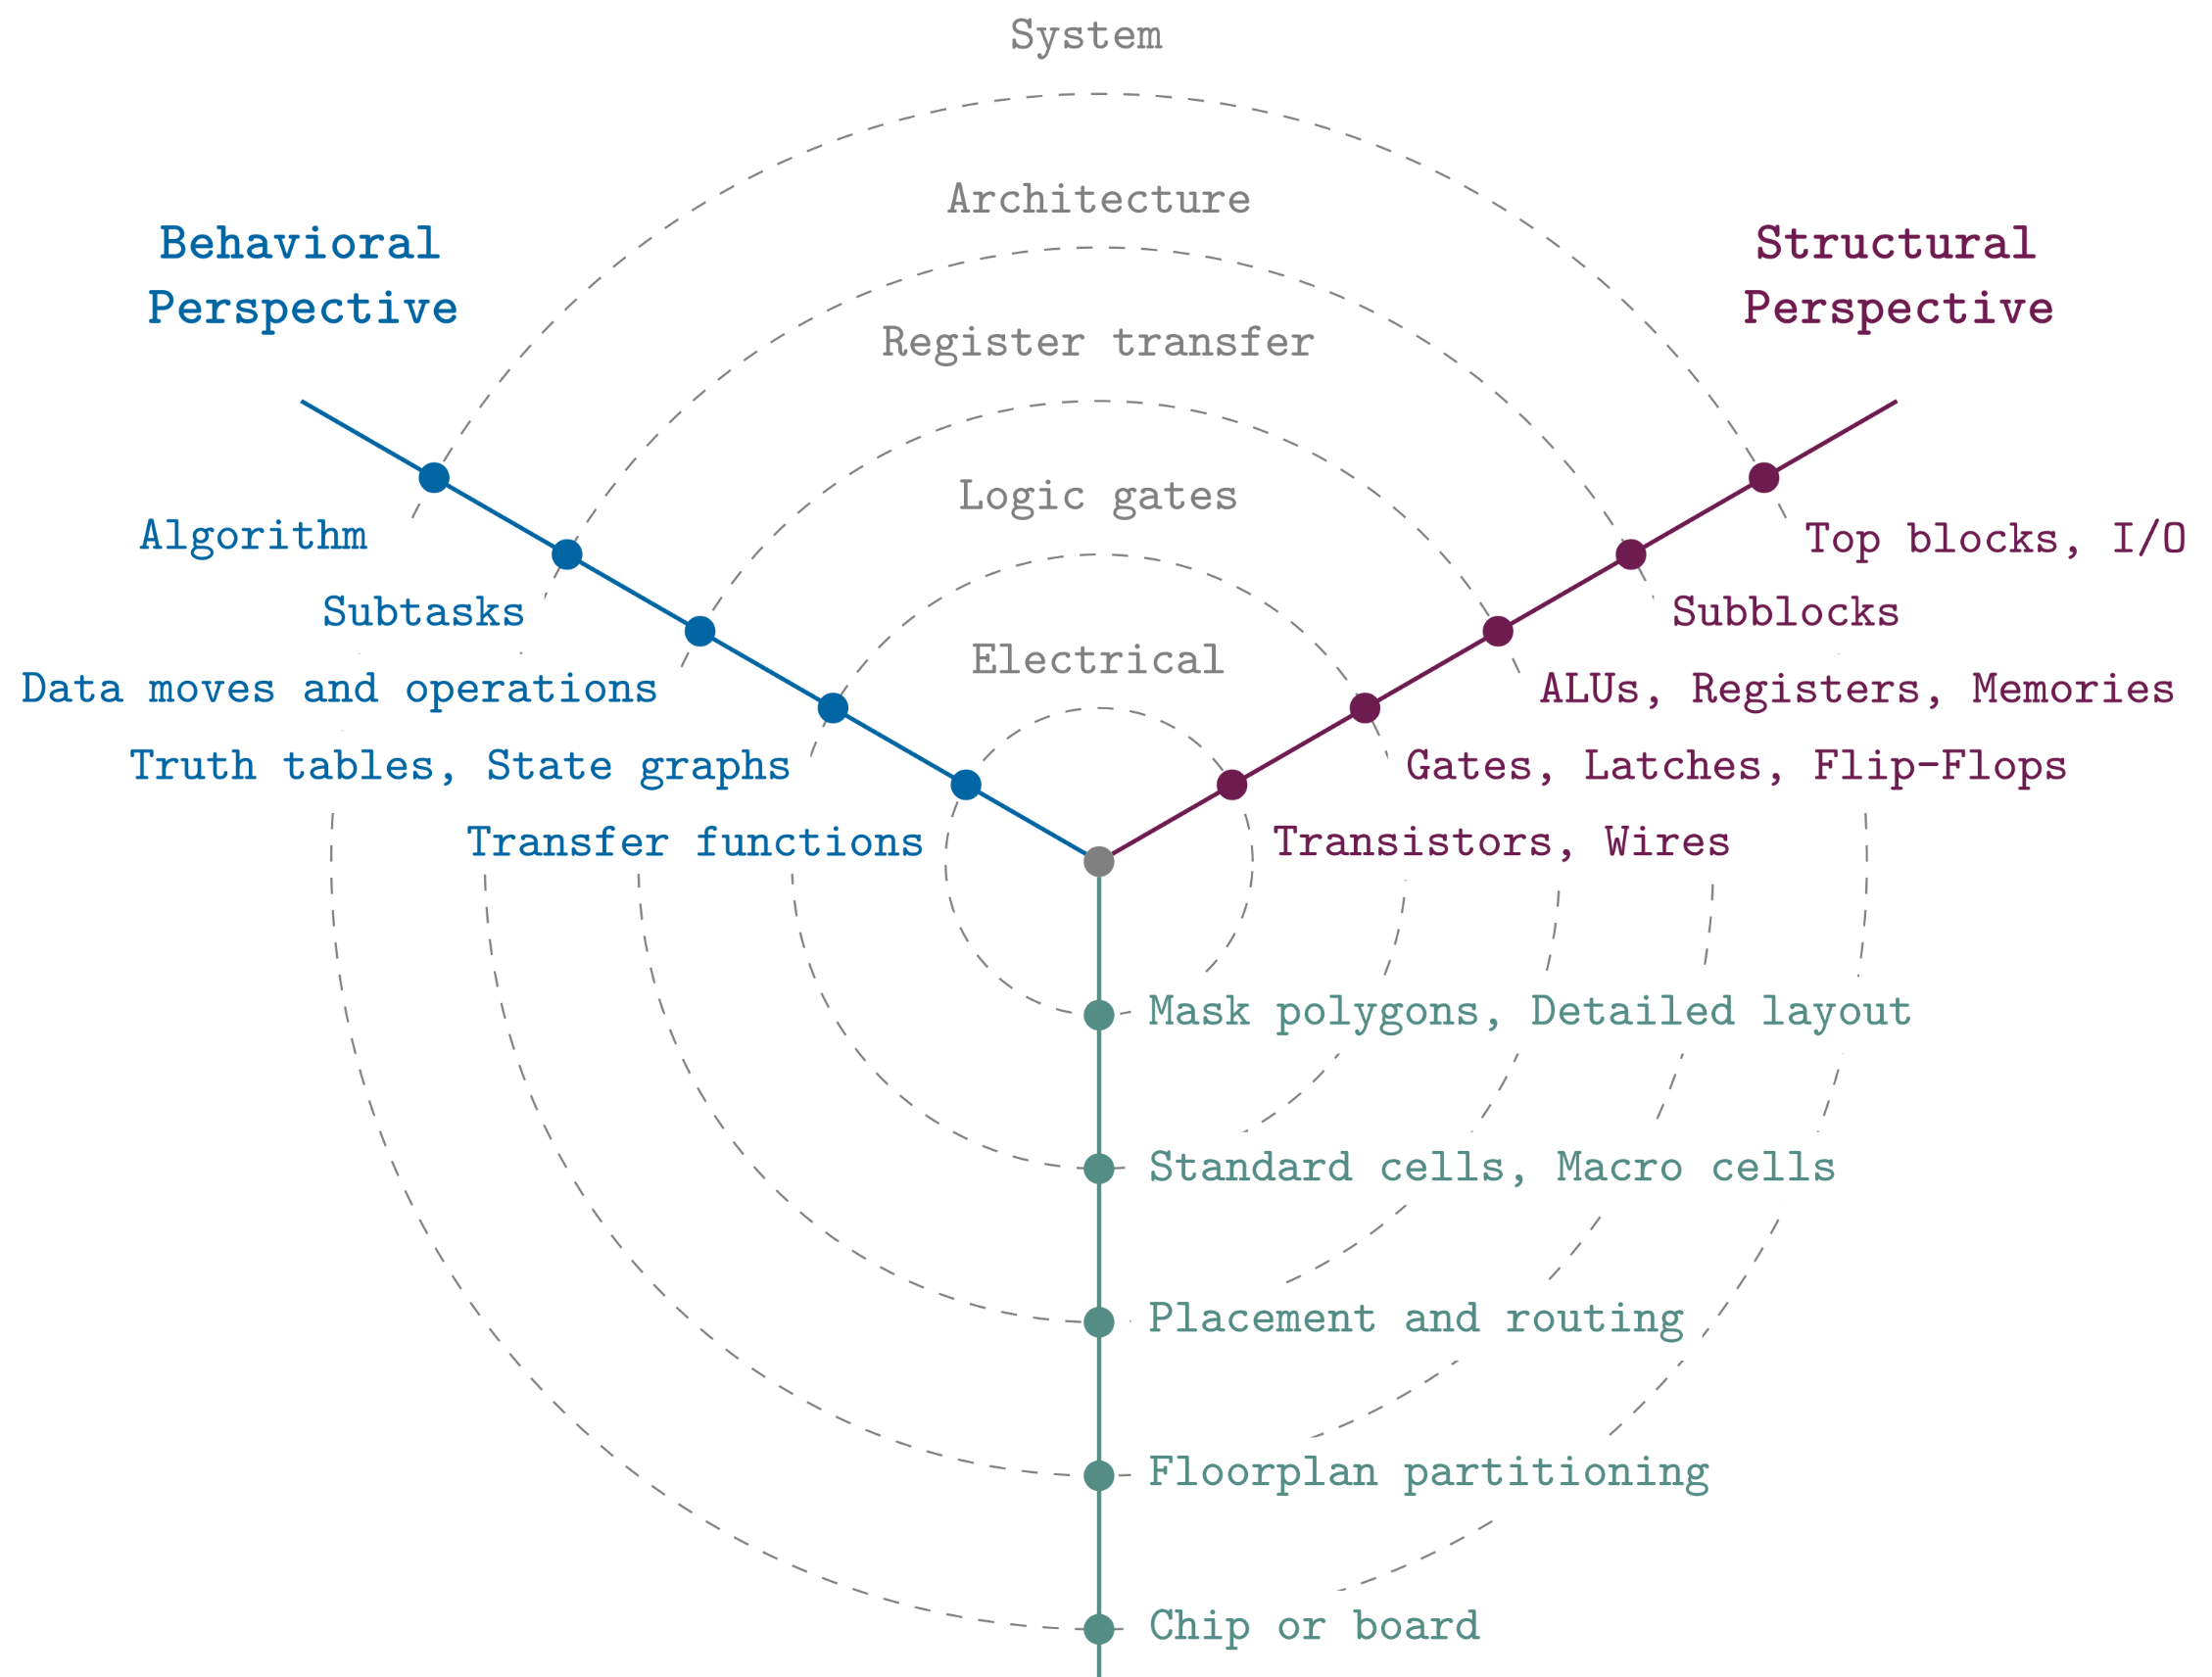
\includegraphics[width=\linewidth]{Images/DevelopmentModel.png}
        \end{minipage}
        \hfill
        \begin{minipage}[t]{0.48\columnwidth}
            \vspace{0pt}  %<-- ensures top alignment
            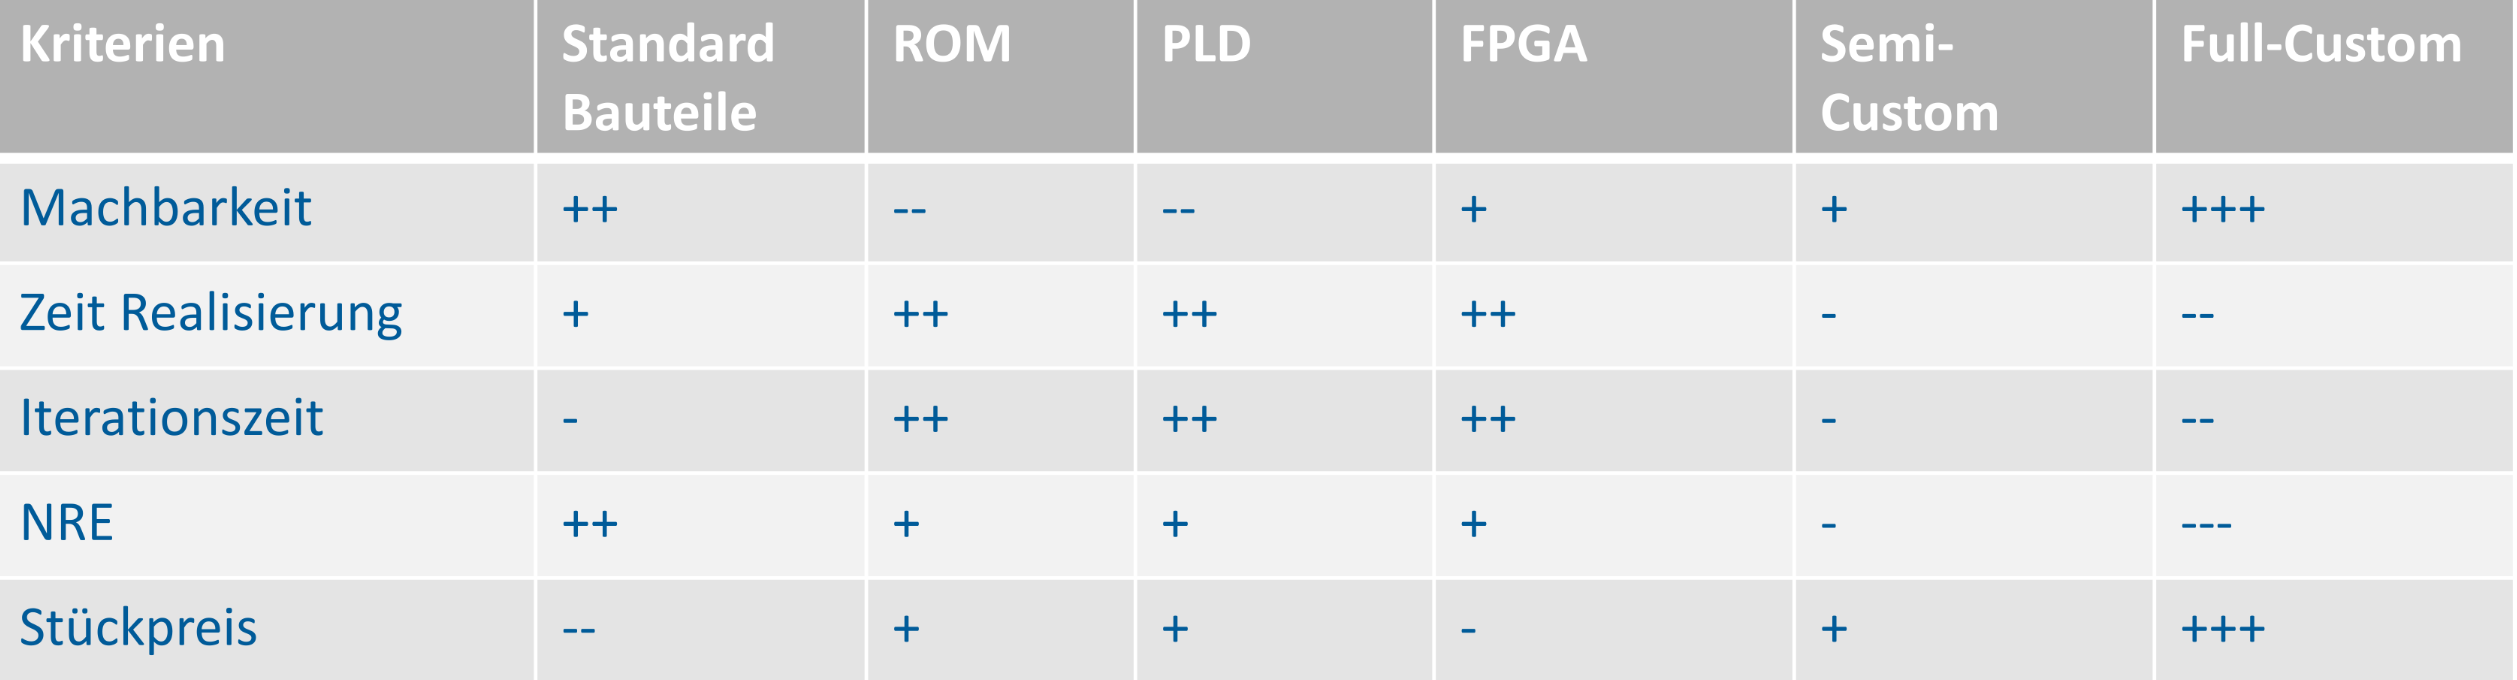
\includegraphics[width=\linewidth]{Images/WhalDerRealisirungsform.png}\\[1ex]
            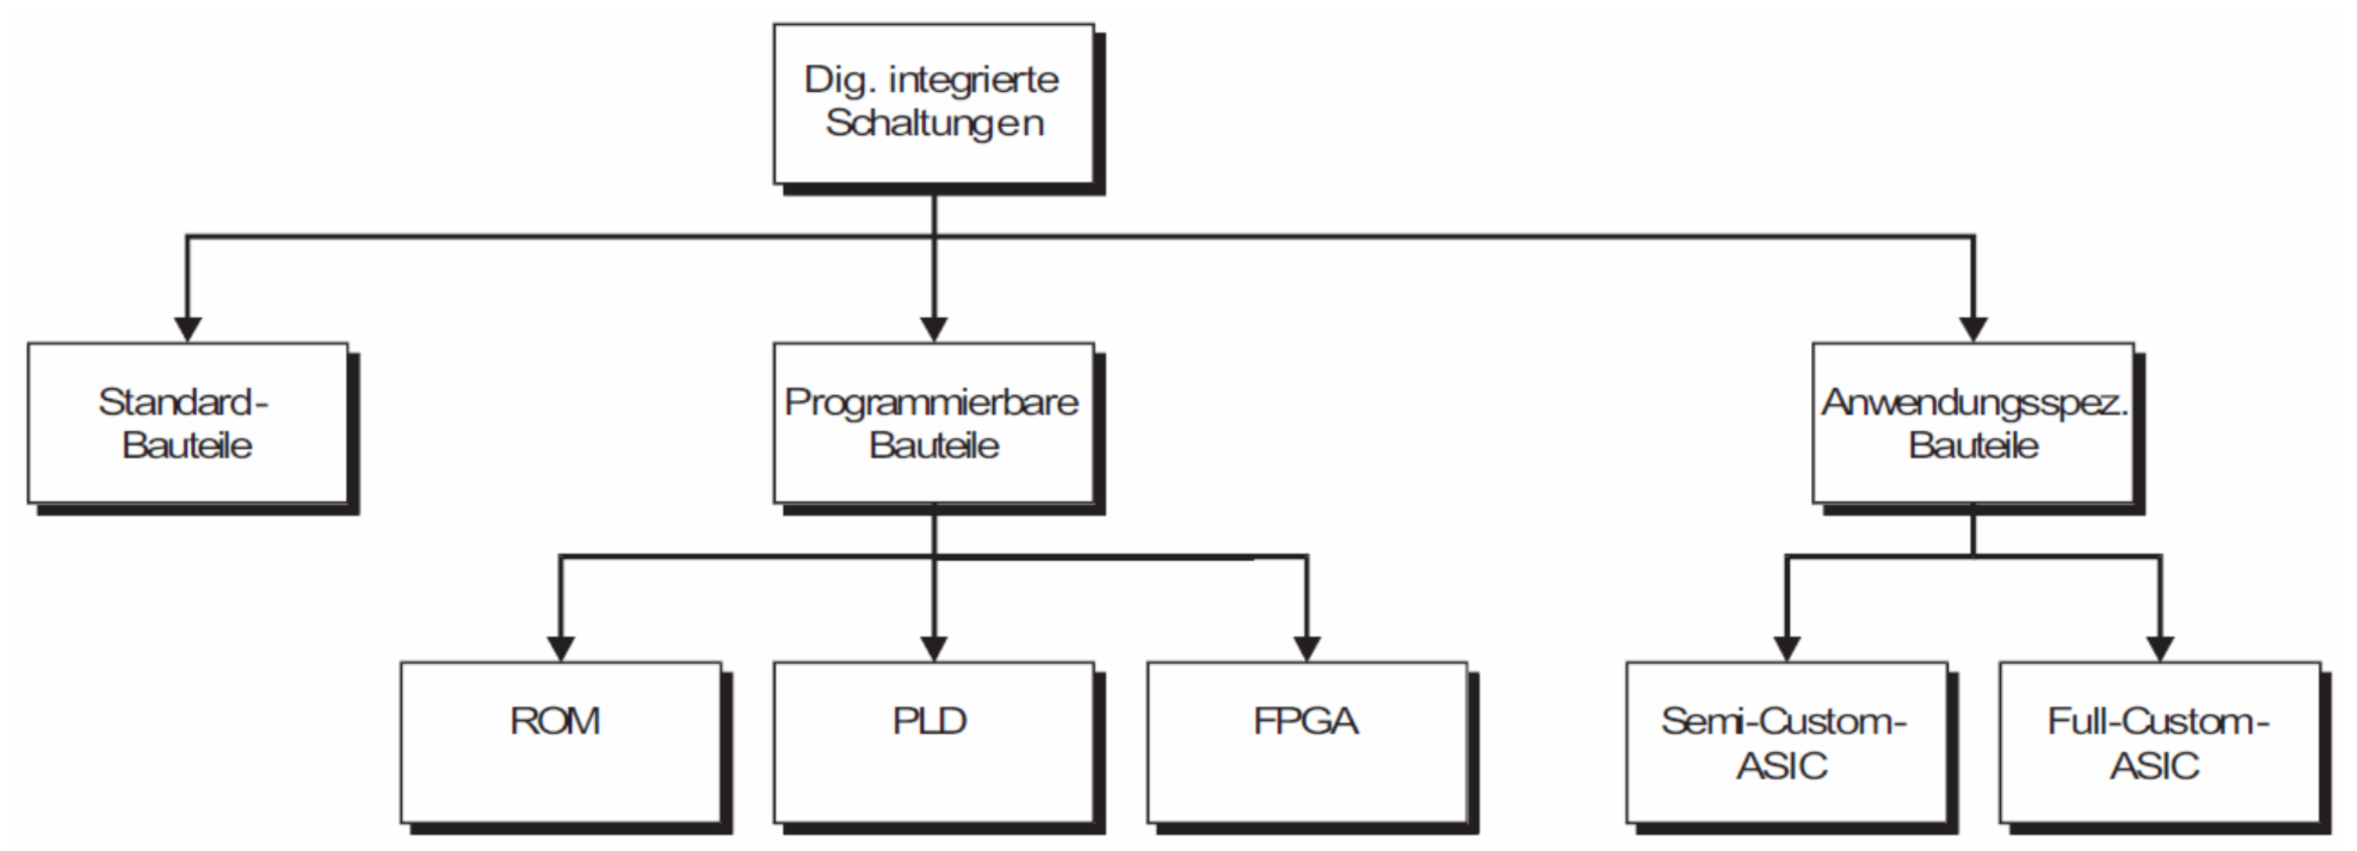
\includegraphics[width=\linewidth]{Images/ClassificationeDeiComponenti.png}
        \end{minipage}


% ==================== DESGIN MUSTER ========================
    \subsection{Guida al design}
        \begin{minipage}[t]{0.48\columnwidth}
            \vspace{0pt} % ensures top alignment
            \begin{enumerate}
                \item Design / Entry
                \item Funktionale Simulation
                \item Synthese
                \item Implementierung
                \begin{itemize}
                    \item Logikoptimierung
                    \item Platzierung
                    \item Verdrahtung
                \end{itemize}
                \item Timing Simulation
                \item Statische Timing Analyse
                \item Herstellungsdatenerzeugen
            \end{enumerate}
        \end{minipage}
        \hfill
        \begin{minipage}[t]{0.48\columnwidth}
            \vspace{0pt} % ensures top alignment
            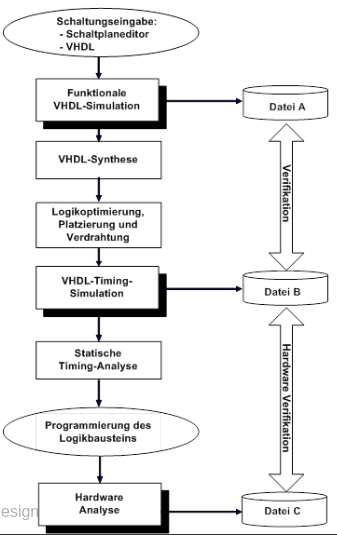
\includegraphics[width=\linewidth]{Images/GuidaDesign.png}
        \end{minipage}


% ==================== BUBBLE DIAGRAM ========================
    \subsection{Bubble diagram}
        \begin{minipage} [t]{0.48\columnwidth}
            \vspace{0pt} % ensures top alignment
            \begin{itemize}
                \item \textbf{Bolle}: Ogni bolla rappresenta uno stato
                \item \textbf{Freccie}: Condizione per passare da uno stato all'altro dev'essere scritta accanto alla freccia.
                \item \textbf{Moore}: Gli output sono associati agli stati, quindi scritti dentro a quest'ultimi.
                \item \textbf{Melay}: Gli output sono associati alle transizioni, quindi scritti accanto alle frecce.
            \end{itemize}
        \end{minipage}
        \begin{minipage} [t]{0.48\columnwidth}
            \vspace{0pt} % ensures top alignment
            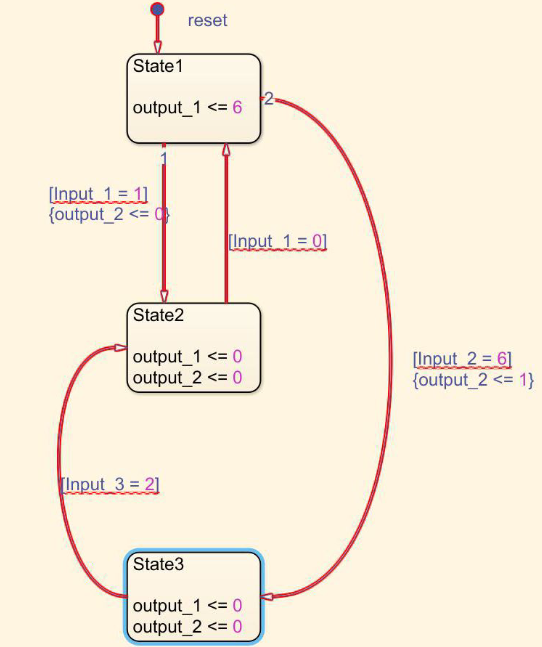
\includegraphics[width=\linewidth]{Images/BubbleDiagram.png}
        \end{minipage}